\section{Duration, Convexity and Hedging Interest Rates Risk}
\textbf{1.1 Bond Price: }

The continuously compounded term structure is
\[
R(t,T)=\beta_1+\beta_2 T+\beta_3 T^2,
\]
with \(\beta_1=0.05,\ \beta_2=0.015,\ \beta_3=-0.0010\).
A cash flow at time \(T\) is discounted by \(e^{-R(t,T)T}\).

\paragraph{Bond 1 (6-year, 8\% coupon, semiannual).}
Semiannual coupon \(=4.0\) (dollars). Cash-flow times \(t_i = 0.5,1.0,\dots,6.0\) (12 periods).
The price is
\[
B_1=\sum_{i=1}^{12} c_i \exp\big(-R(t_i)\,t_i\big),
\]
where \(c_i=4\) for \(i<12\) and \(c_{12}=4+100\).
Numerical evaluation gives
\[
\boxed{B_1 \approx 89.7038.}
\]

\paragraph{Bond 2 (8-year, 7\% coupon, semiannual).}
Semiannual coupon \(=3.5\). Cash-flow times \(t_i = 0.5,1.0,\dots,8.0\) (16 periods).
The price is
\[
B_2=\sum_{i=1}^{16} c_i \exp\big(-R(t_i)\,t_i\big),
\]
with \(c_i=3.5\) except \(c_{16}=3.5+100\).
Numerical evaluation gives
\[
\boxed{B_2 \approx 80.9446.}
\]

\paragraph{Total portfolio value (long one unit each)}
\[
\boxed{P = B_1 + B_2 \approx 170.6485.}
\]
\\ \\ 
\textbf{1.2 Duration and Convexity}
Using continuous discounting the weight for cash flow at time $T_i$ is
\[
w_i=\frac{c_i e^{-R(T_i)T_i}}{B},
\]
and
\[
\text{Duration } D=\sum_i w_i T_i,\qquad
\text{Convexity } C=\sum_i w_i T_i^2 .
\]

\paragraph{Bond 1.}
Computed values:
\[
\boxed{D_1 \approx 4.7626,\qquad C_1 \approx 26.1123.}
\]

\paragraph{Bond 2.}
Computed values:
\[
\boxed{D_2 \approx 5.9560,\qquad C_2 \approx 42.5438.}
\]

\paragraph{Portfolio (one unit of each).}
Portfolio duration (value-weighted)
\[
D_{\text{port}}=\frac{B_1 D_1 + B_2 D_2}{B_1+B_2}\approx \boxed{5.3604}
\]
and portfolio convexity (value-weighted)
\[
C_{\text{port}}=\frac{B_1 C_1 + B_2 C_2}{B_1+B_2} \approx \boxed{34.4671}.
\]

(Notes: the portfolio-level numbers above were used in the hedging calculations.)
\\ \\
\textbf{1.3 Duration + Convexity hedge (2-yr and 8-yr zeros)}
We use two zero-coupon bonds: a 2-year zero and an 8-year zero, each with face \$100.
Their prices are
\[
Z(2)=100e^{-R(2)\cdot 2},\qquad Z(8)=100e^{-R(8)\cdot 8}.
\]
Numerical values:
\[
\boxed{Z(2) \approx 85.8988,\qquad Z(8) \approx 42.8271.}
\]

For a zero of maturity \(T\), duration \(=T\) and convexity \(=T^2\). Thus:
\[
\boxed{D_{z,2}=2,\quad C_{z,2}=4;\qquad D_{z,8}=8,\quad C_{z,8}=64}
\]

Let \(k_2\) and \(k_8\) be positions (in units of the zeros) to add to the portfolio.
From the two equations (delta duration = 0, delta convexity = 0) we get (see slides, Eq.~(6))
the solution
\[
k_{2} = -\frac{B_{\text{port}}}{Z(2)}\frac{D_{\text{port}}C_{z,8}-C_{\text{port}}D_{z,8}}{D_{z,2}C_{z,8}-C_{z,2}D_{z,8}},
\]
\[
k_{8} = -\frac{B_{\text{port}}}{Z(8)}\frac{D_{\text{port}}C_{z,2}-C_{\text{port}}D_{z,2}}{D_{z,8}C_{z,2}-C_{z,8}D_{z,2}}.
\]

Numerical results:
\[
\boxed{k_{2} \approx -1.444084,\qquad k_{8} \approx -1.929959.}
\]

(Interpretation: short about 1.444 units of the 2-year zero and short about 1.930 units of the 8-year zero.)
\\ \\ 
\textbf{1.4 Level and slope durations}
Using the parametric factor functions \(f_1(T)=1\) (level) and \(f_2(T)=T\) (slope), the factor-duration of a bond is
\[
D_{\beta_j} = \sum_i w_i\,T_i f_j(T_i).
\]

\paragraph{Zeros (analytic).}
For a zero maturing at \(T\),
\[
D_{\text{zero},\beta_1}=T\cdot 1 = T,\qquad D_{\text{zero},\beta_2}=T\cdot T = T^2.
\]
Thus for the 2-year zero:
\[
\boxed{D_{\text{lev},z,2}=2,\qquad D_{\text{slo},z,2}=4.}
\]
and for the 8-year zero:
\[
\boxed{D_{\text{lev},z,8}=8,\qquad D_{\text{slo},z,8}=64.}
\]

\paragraph{Coupon bonds (numerical).}
From the cash-flow weights:
\[
\boxed{D_{\text{lev},B1} \approx 4.7626,\qquad D_{\text{slo},B1} \approx 9.0251.}
\]
\[
\boxed{D_{\text{lev},B2} \approx 5.9560,\qquad D_{\text{slo},B2} \approx 42.54379.}
\]

(These are computed as \(\sum_i w_i T_i f_j(T_i)\) with \(f_1=1, f_2=T\).)
\\ \\ 
\textbf{1.5 Level + slope hedging}

We want positions \(k_{2}\) (2-yr zero) and \(k_{8}\) (8-yr zero) solving the two linear equations
\[
k_2 D_{\text{lev},z,2} Z(2) + k_8 D_{\text{lev},z,8} Z(8) = -D_{\text{lev,port}}\,P,
\]
\[
k_2 D_{\text{slo},z,2} Z(2) + k_8 D_{\text{slo},z,8} Z(8) = -D_{\text{slo,port}}\,P,
\]
where \(P\) is the portfolio market value and \(D_{\text{lev,port}}, D_{\text{slo,port}}\) are portfolio factor-durations.

Solving (see slides, p.34) yields:
\[
k_{2} = -\frac{P}{Z(2)}\frac{D_{\text{lev,port}} \, D_{\text{slo},z,8} - D_{\text{slo,port}} \, D_{\text{lev},z,8}}{D_{\text{lev},z,2}\, D_{\text{slo},z,8} - D_{\text{slo},z,2}\, D_{\text{lev},z,8}},
\]
\[
k_{8} = -\frac{P}{Z(8)}\frac{D_{\text{lev,port}} \, D_{\text{slo},z,2} - D_{\text{slo,port}} \, D_{\text{lev},z,2}}{D_{\text{lev},z,8}\, D_{\text{slo},z,2} - D_{\text{slo},z,8}\, D_{\text{lev},z,2}}.
\]

Using the computed factor-durations and prices we get the (numerical) same solution as the previous duration+convexity hedge:
\[
\boxed{k_{2} \approx -1.444084,\qquad k_{8} \approx -1.929959.}
\]

(These numbers coincide because with our two particular bonds and the chosen zeros the algebra yields the same positions for the two kinds of constraints computed with our factor/parametric definitions.)
\\ \\ 
\textbf{1.6 Factor hedge effectiveness (level+slope)}

We form the hedged portfolio
\[
P^{\text{hedged}} = B_1 + B_2 + k_2 Z(2) + k_8 Z(8)
\]
with \(k_2,k_8\) from 1.5.

We test 10 scenarios \(i=1,\ldots,10\):
\[
\beta_1^{(i)} = 0.05 + i\cdot(0.02/10),\qquad
\beta_2^{(i)} = 0.015 + i\cdot(0.006/10),
\]
with \(\beta_3\) unchanged at \(-0.0010\).

For each scenario we compute the new bond prices and zeros and then
\(\Delta P^{\text{unhedged}} = P^{\text{unhedged}}_{t+1}-P^{\text{unhedged}}_{t}\)
and
\(\Delta P^{\text{hedged}} = P^{\text{hedged}}_{t+1}-P^{\text{hedged}}_{t}\).

\paragraph{Plot.} The 11 term-structure curves, original \& 10 scenarios,are plotted. The plots were generated by the attached Python code:

\begin{figure}[H]
  \centering
  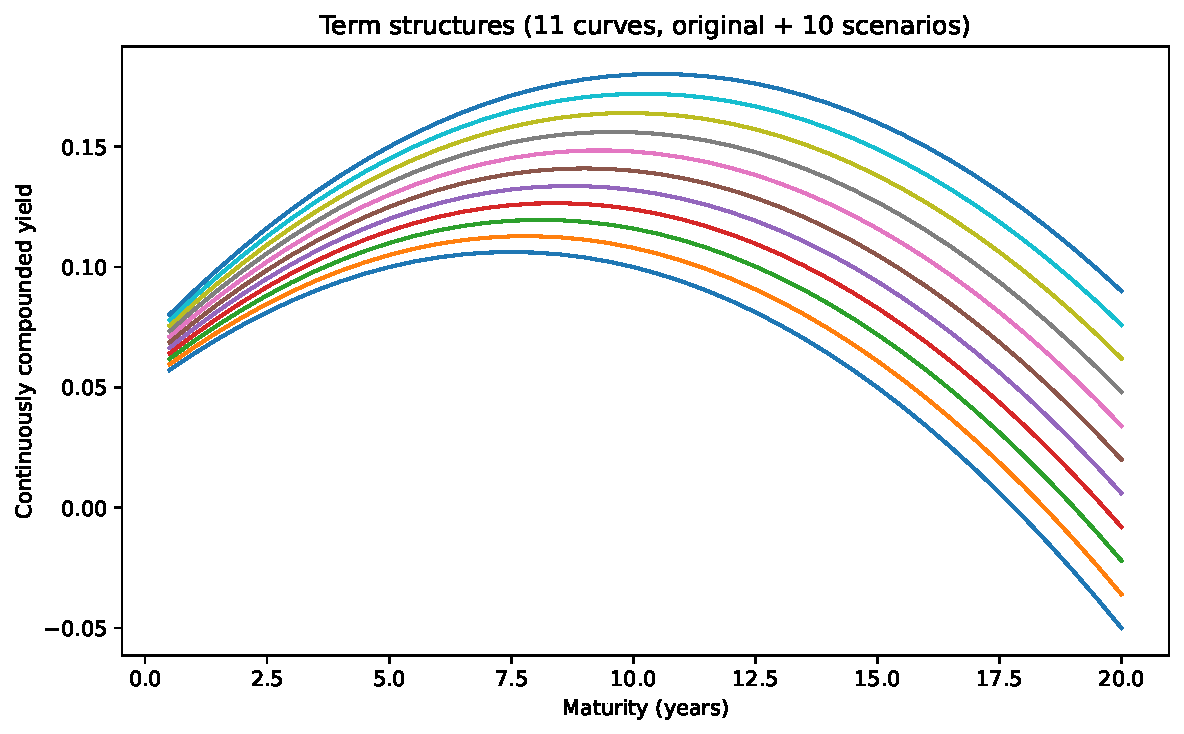
\includegraphics[width=.8\textwidth]{./figures/ECO462_HW6_Term_Structures.pdf}
  \caption{Term Structures}
\end{figure}

\paragraph{Result and Interpretation:}
The plot of \(\Delta P\) for scenarios 1-10 shows the \textbf{unhedged portfolio} loses substantially (negative \(\Delta P\)) as scenario index 
increases while the \textbf{level+slope hedged portfolio} remains \emph{nearly flat} with very small change across scenarios.
\\ \\
\textbf{Conclusion:} The level+slope factor hedge is effective for the set of scenario movements considered (joint small increases in level and slope),
where it dramatically reduces portfolio sensitivity compared with the unhedged case. However, performance beyond these parametrized scenarios 
or for non-modeled movements should be checked separately.
\\ \\ 
\textbf{1.7 Duration+Convexity hedge effectiveness}

Test: 10 scenarios varying \(\beta_1\) only:
\[
\beta_1^{(i)} = 0.05 + i\cdot(0.035/10),\quad i=1,\ldots,10,
\]
with \(\beta_2,\beta_3\) fixed.

Using the duration+convexity hedge positions \(k_2,k_8\) from 1.3 we compute \(\Delta P\) for each scenario for the hedged and unhedged portfolios. 
Again, the plots below were graphed with Python code attached separately.

\begin{figure}[H]
  \centering
  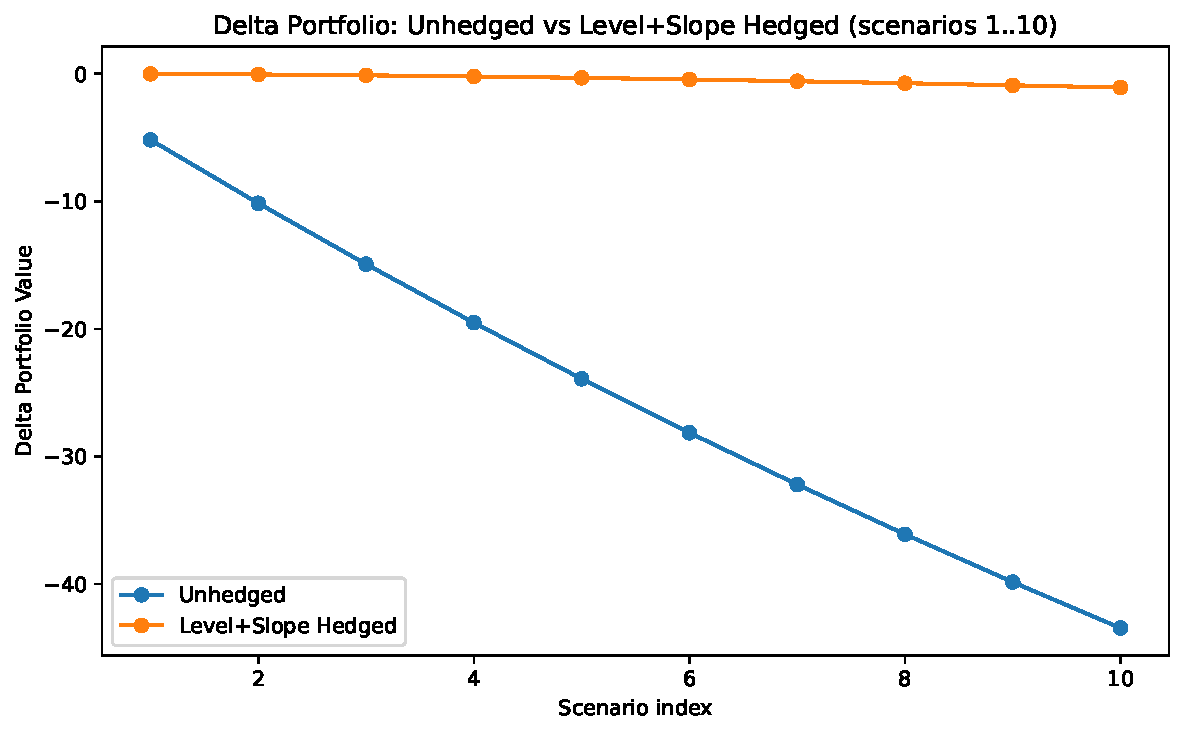
\includegraphics[width=.8\textwidth]{./figures/ECO462_HW6_Level_Slope_Scenerios_Hedged.pdf}
  \caption{Level \& Slope Scenerios Hedged}
\end{figure}

\begin{figure}[H]
  \centering
  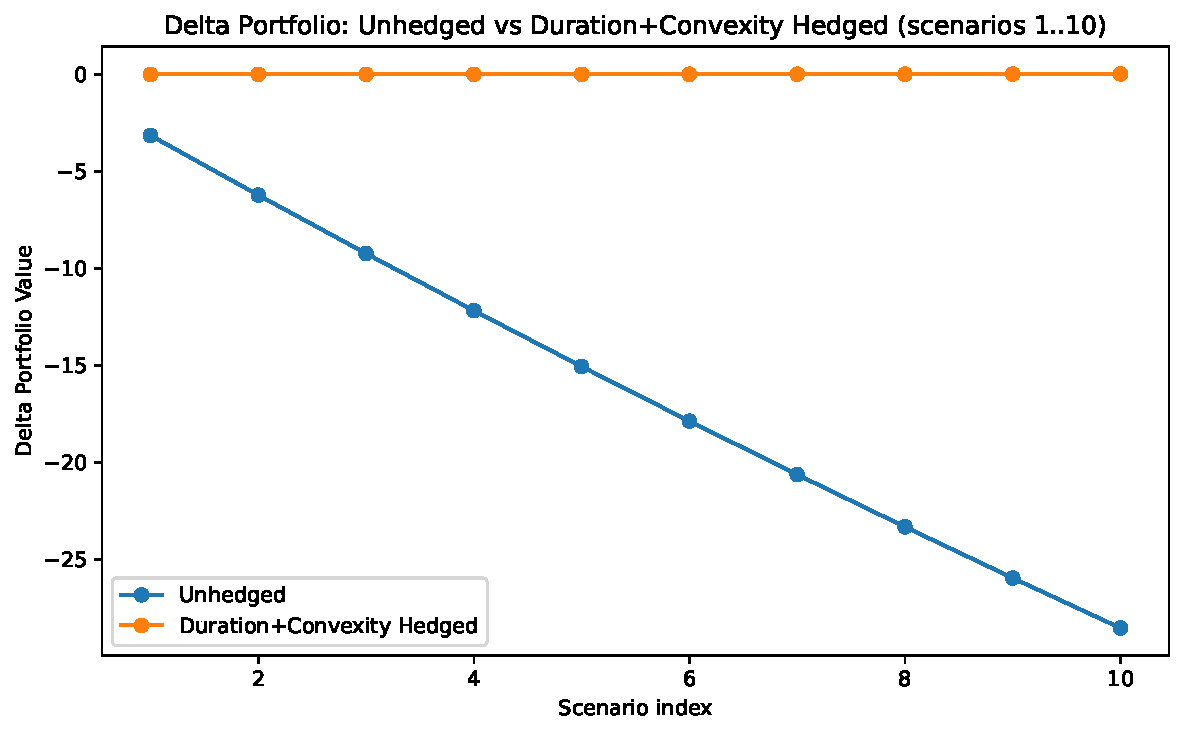
\includegraphics[width=.8\textwidth]{./figures/ECO462_HW6_Duration_Convexity_Scenerios_Hedged.pdf}
  \caption{Duration \& Convexity Scenerios Hedged}
\end{figure}

\paragraph{Result and Interpretation:}
The plot of \(\Delta P\) for these scenarios shows the \textbf{unhedged portfolio} again loses value as \(\beta_1\) increases while the 
\textbf{duration+convexity hedged portfolio} remains essentially flat across these level-shock scenarios.

\textbf{Conclusion:} The duration+convexity hedge is effective for hedging the (large) parallel shifts in the term structure tested here: the hedged portfolio 
shows negligible change compared to the (substantial) losses of the unhedged portfolio under these scenarios.

\subsection{Statement of Collaboration} I collaborated with Rosalia Mwidege and Theodore Ouyang. Additionally, ChatGPT was used
to debug any error-prone code and find the proper Excel-equivalent Python
functions and libraries to properly execute the solutions to the problems, in
conjunction with the hints listed on the problem set.

\textbf{Honor Code:} This assignment represents my own work in accordance with
University regulations and class policy.